\documentclass{article}
\usepackage{tikz}
\usepackage{geometry}
\usepackage[dvipsnames]{xcolor}
\pagestyle{empty}

\newcommand{\docpaperwidth}{12.8cm}
\newcommand{\docpaperheight}{9.6cm}

\geometry{
  papersize={\docpaperwidth,\docpaperheight},
  margin=0cm,
  ignoreall=true
}
\usetikzlibrary{backgrounds}
\usetikzlibrary{shapes.geometric}

\pgfdeclareimage[width=12.8cm]{hwfront01}{aiopcwa-front-1.jpg}
\pgfdeclareimage[width=12.8cm]{hwback01}{aiopcwa-back-1.jpg}
\pgfdeclareimage[width=12.8cm]{hwinternal}{aiopcwa-internal-1.jpg}
\pgfdeclareimage[width=12.8cm]{hwinsusb0}{aiopcwa-insert-usb-0.jpg}
\pgfdeclareimage[width=12.8cm]{hwinsusb1}{aiopcwa-insert-usb-1.jpg}
\pgfdeclareimage[width=12.8cm]{hwinsusb2}{aiopcwa-insert-usb-2.jpg}

\setlength{\parindent}{0cm}

\begin{document}
  % plane front image
  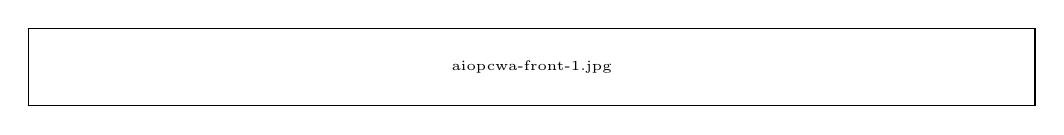
\begin{tikzpicture}
    \begin{scope}[on background layer]
      \pgftext[at=\pgfpoint{0cm}{0cm},left,base]{\pgfuseimage{hwfront01}}
    \end{scope}
  \end{tikzpicture}
  \newpage
  % plane back image
  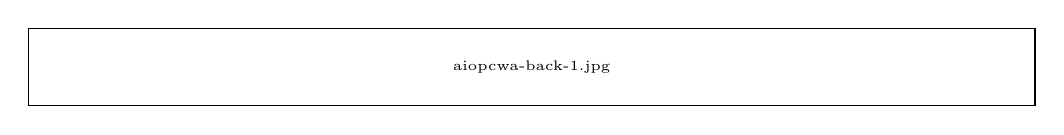
\begin{tikzpicture}
    \begin{scope}[on background layer]
      \pgftext[at=\pgfpoint{0cm}{0cm},left,base]{\pgfuseimage{hwback01}}
    \end{scope}
  \end{tikzpicture}
  \newpage
  % mark usb3.2 on front image
  \begin{tikzpicture}
    \newcommand{\eclivecf}{\pgfpoint{0.5cm}{0cm}}
    \newcommand{\eclivecs}{\pgfpoint{0cm}{0.25cm}}
    \color{YellowOrange}
    \pgfsetlinewidth{2pt} 
    \pgfpathellipse{\pgfpoint{6.15cm}{2.65cm}}
      {\eclivecf}
      {\eclivecs}
    \pgfpathellipse{\pgfpoint{7.4cm}{2.65cm}}
      {\eclivecf}
      {\eclivecs}
    \pgfusepath{draw}
    \begin{scope}[on background layer]
      \pgftext[at=\pgfpoint{0cm}{0cm},left,base]{\pgfuseimage{hwfront01}}
    \end{scope}
  \end{tikzpicture}
  \newpage
  % mark usb 2.0 on back image
  \begin{tikzpicture}
    \newcommand{\eclivecf}{\pgfpoint{0.5cm}{0cm}}
    \newcommand{\eclivecs}{\pgfpoint{0cm}{0.25cm}}
    \color{YellowOrange}
    \pgfsetlinewidth{2pt} 
    \pgfpathellipse{\pgfpoint{2.85cm}{3.55cm}}
      {\eclivecf}
      {\eclivecs}
    \pgfpathellipse{\pgfpoint{2.75cm}{4cm}}
      {\eclivecf}
      {\eclivecs}
    \pgfusepath{draw}
    \begin{scope}[on background layer]
      \pgftext[at=\pgfpoint{0cm}{0cm},left,base]{\pgfuseimage{hwback01}}
    \end{scope}
  \end{tikzpicture}
  \newpage
  % mark DP 2.1 on back image
  \begin{tikzpicture}
    \newcommand{\eclivecf}{\pgfpoint{0.5cm}{0cm}}
    \newcommand{\eclivecs}{\pgfpoint{0cm}{0.25cm}}
    \color{YellowOrange}
    \pgfsetlinewidth{2pt} 
    \pgfpathellipse{\pgfpoint{6.65cm}{4.08cm}}
      {\eclivecf}
      {\eclivecs}
    \pgfpathellipse{\pgfpoint{8.2cm}{4.08cm}}
      {\eclivecf}
      {\eclivecs}
    \pgfusepath{draw}
    \begin{scope}[on background layer]
      \pgftext[at=\pgfpoint{0cm}{0cm},left,base]{\pgfuseimage{hwback01}}
    \end{scope}
  \end{tikzpicture}
  \newpage
  % mark DP 2.1 on back image
  \begin{tikzpicture}
    \newcommand{\eclivecf}{\pgfpoint{0.5cm}{0cm}}
    \newcommand{\eclivecs}{\pgfpoint{0cm}{0.25cm}}
    \color{YellowOrange}
    \pgfsetlinewidth{2pt} 
    \pgfpathellipse{\pgfpoint{6.65cm}{3.5cm}}
      {\eclivecf}
      {\eclivecs}
    \pgfpathellipse{\pgfpoint{8cm}{3.5cm}}
      {\eclivecf}
      {\eclivecs}
    \pgfusepath{draw}
    \begin{scope}[on background layer]
      \pgftext[at=\pgfpoint{0cm}{0cm},left,base]{\pgfuseimage{hwback01}}
    \end{scope}
  \end{tikzpicture}
  \newpage
  % mark Serial Port on back image
  \begin{tikzpicture}
    \newcommand{\eclivecf}{\pgfpoint{0.6cm}{0cm}}
    \newcommand{\eclivecs}{\pgfpoint{0cm}{0.3cm}}
    \color{YellowOrange}
    \pgfsetlinewidth{2pt} 
    \pgfpathellipse{\pgfpoint{4.65cm}{2.8cm}}
      {\eclivecf}
      {\eclivecs}
    \pgfusepath{draw}
    \begin{scope}[on background layer]
      \pgftext[at=\pgfpoint{0cm}{0cm},left,base]{\pgfuseimage{hwback01}}
    \end{scope}
  \end{tikzpicture}
  \newpage
  % mark LAN on back image
  \begin{tikzpicture}
    \newcommand{\eclivecf}{\pgfpoint{0.5cm}{0cm}}
    \newcommand{\eclivecs}{\pgfpoint{0cm}{0.25cm}}
    \color{YellowOrange}
    \pgfsetlinewidth{2pt} 
    \pgfpathellipse{\pgfpoint{4cm}{3.9cm}}
      {\eclivecf}
      {\eclivecs}
    \pgfpathellipse{\pgfpoint{5.3cm}{3.9cm}}
      {\eclivecf}
      {\eclivecs}
    \pgfusepath{draw}
    \begin{scope}[on background layer]
      \pgftext[at=\pgfpoint{0cm}{0cm},left,base]{\pgfuseimage{hwback01}}
    \end{scope}
  \end{tikzpicture}
  % mark WI-FI antenna on back image
  
\begin{tikzpicture}
    \newcommand{\vecrota}{103}
    \newcommand{\vecrotb}{68}
    \newcommand{\vecafx}{1.5cm}
    \newcommand{\vecafy}{0cm}
    \newcommand{\vecasx}{0cm}
    \newcommand{\vecasy}{0.4cm}

    \newcommand{\vecbfx}{1.5cm}
    \newcommand{\vecbfy}{0cm}
    \newcommand{\vecbsx}{0cm}
    \newcommand{\vecbsy}{0.4cm}

    \newcommand{\vecrotatex}[3]{
      cos(#3)  * #1 - sin(#3) * #2
    }
    \newcommand{\vecrotatey}[3]{
      sin(#3) * #1 + cos(#3) * #2
    }
    \newcommand{\ellivecaf}{
      \pgfpoint{\vecrotatex{\vecafx}{\vecafy}{\vecrota}}
        {\vecrotatey{\vecafx}{\vecafy}{\vecrota}}}
    \newcommand{\ellivecas}{
      \pgfpoint{\vecrotatex{\vecasx}{\vecasy}{\vecrota}}
        {\vecrotatey{\vecasx}{\vecasy}{\vecrota}}}
    \newcommand{\ellivecbf}{
      \pgfpoint{\vecrotatex{\vecbfx}{\vecbfy}{\vecrotb}}
        {\vecrotatey{\vecbfx}{\vecbfy}{\vecrotb}}}
    \newcommand{\ellivecbs}{
      \pgfpoint{\vecrotatex{\vecbsx}{\vecbsy}{\vecrotb}}
        {\vecrotatey{\vecbsx}{\vecbsy}{\vecrotb}}}
    \color{YellowOrange}
    \pgfsetlinewidth{2pt} 
    \pgfpathellipse{\pgfpoint{1.3cm}{3.5cm}}
      {\ellivecaf}
      {\ellivecas}
    \pgfpathellipse{\pgfpoint{11cm}{3.5cm}}
      {\ellivecbf}
      {\ellivecbs}
    \pgfusepath{draw}
    \begin{scope}[on background layer]
      \pgftext[at=\pgfpoint{0cm}{0cm},left,base]{\pgfuseimage{hwback01}}
    \end{scope}
  \end{tikzpicture}
  \newpage
  % usb inserted image 0
  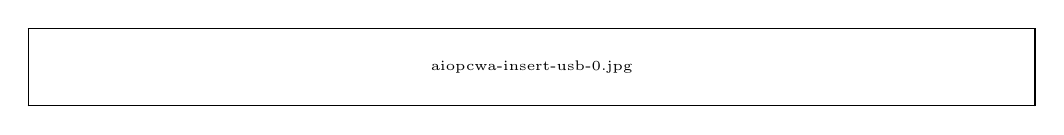
\begin{tikzpicture}
    \begin{scope}[on background layer]
      \pgftext[at=\pgfpoint{0cm}{0cm},left,base]{\pgfuseimage{hwinsusb0}}
    \end{scope}
  \end{tikzpicture}
  \newpage
  % usb inserted image 1-1
  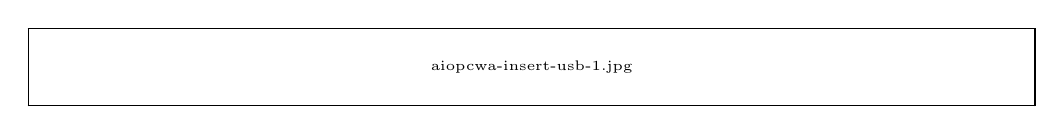
\begin{tikzpicture}
    \begin{scope}[on background layer]
      \pgftext[at=\pgfpoint{0cm}{0cm},left,base]{\pgfuseimage{hwinsusb1}}
    \end{scope}
  \end{tikzpicture}
  \newpage
  % usb inserted image 1-2
  \begin{tikzpicture}
    \newcommand{\rw}{1.3cm}
    \newcommand{\rh}{2.3cm}
    \newcommand{\rox}{6.52cm}
    \newcommand{\roy}{2.8cm}
    \newcommand{\lfx}{0cm} %left far x
    \newcommand{\lnx}{0.1cm} %left near x
    \newcommand{\rfx}{0cm} %right far x
    \newcommand{\rnx}{0.1cm} %right near x

    \newcommand{\pa}{\pgfpoint{\rox - (\rw + \lnx + \lfx) / 2}{\roy}}
    \newcommand{\pb}{\pgfpoint{\rox - \rw / 2 - \lnx}{\roy - \rh / 2}}
    \newcommand{\pc}{\pgfpoint{\rox + \rw / 2 + \rnx}{\roy - \rh / 2}}
    \newcommand{\pd}{\pgfpoint{\rox + \rw / 2 + \rfx}{\roy + \rh / 2}}
    \newcommand{\pe}{\pgfpoint{\rox - \rw / 2 - \lfx}{\roy + \rh / 2}}

    \pgfsetcornersarced{\pgfpoint{1mm}{1mm}}
    \pgfpathmoveto{\pa}
    \pgfpathlineto{\pb}
    \pgfpathlineto{\pc}
    \pgfpathlineto{\pd}
    \pgfpathlineto{\pe}
    \pgfpathclose
    \color{YellowOrange}
    \pgfsetlinewidth{2pt} 
    \pgfusepath{draw}
    \begin{scope}[on background layer]
      \pgftext[at=\pgfpoint{0cm}{0cm},left,base]{\pgfuseimage{hwinsusb1}}
    \end{scope}
  \end{tikzpicture}
  \newpage
  % internal-image
  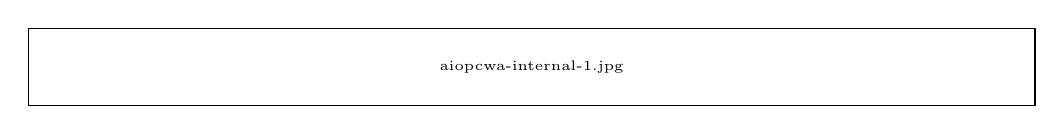
\begin{tikzpicture}
    \begin{scope}[on background layer]
      \pgftext[at=\pgfpoint{0cm}{0cm},left,base]{\pgfuseimage{hwinternal}}
    \end{scope}
  \end{tikzpicture}
  \newpage
  % internal-image mark ssd
  \begin{tikzpicture}
    \newcommand{\rw}{1.3cm}
    \newcommand{\rh}{3.8cm}
    \newcommand{\rox}{3.5cm}
    \newcommand{\roy}{5.15cm}

    \newcommand{\pa}{\pgfpoint{\rox - \rw / 2}{\roy}}
    \newcommand{\pb}{\pgfpoint{\rox - \rw / 2}{\roy - \rh / 2}}
    \newcommand{\pc}{\pgfpoint{\rox + \rw / 2}{\roy - \rh / 2}}
    \newcommand{\pd}{\pgfpoint{\rox + \rw / 2}{\roy + \rh / 2}}
    \newcommand{\pe}{\pgfpoint{\rox - \rw / 2}{\roy + \rh / 2}}

    \pgfsetcornersarced{\pgfpoint{1mm}{1mm}}
    \pgfpathmoveto{\pa}
    \pgfpathlineto{\pb}
    \pgfpathlineto{\pc}
    \pgfpathlineto{\pd}
    \pgfpathlineto{\pe}
    \pgfpathclose
    \color{YellowOrange}
    \pgfsetlinewidth{2pt} 
    \pgfusepath{draw}
    \begin{scope}[on background layer]
      \pgftext[at=\pgfpoint{0cm}{0cm},left,base]{\pgfuseimage{hwinternal}}
    \end{scope}
  \end{tikzpicture}
  \newpage
  % internal-image mark memory
  \begin{tikzpicture}
    \newcommand{\rw}{1.8cm}
    \newcommand{\rh}{3.5cm}
    \newcommand{\rox}{7.78cm}
    \newcommand{\roy}{5.25cm}

    \newcommand{\pa}{\pgfpoint{\rox - \rw / 2}{\roy}}
    \newcommand{\pb}{\pgfpoint{\rox - \rw / 2}{\roy - \rh / 2}}
    \newcommand{\pc}{\pgfpoint{\rox + \rw / 2}{\roy - \rh / 2}}
    \newcommand{\pd}{\pgfpoint{\rox + \rw / 2}{\roy + \rh / 2}}
    \newcommand{\pe}{\pgfpoint{\rox - \rw / 2}{\roy + \rh / 2}}

    \pgfsetcornersarced{\pgfpoint{1mm}{1mm}}
    \pgfpathmoveto{\pa}
    \pgfpathlineto{\pb}
    \pgfpathlineto{\pc}
    \pgfpathlineto{\pd}
    \pgfpathlineto{\pe}
    \pgfpathclose
    \color{YellowOrange}
    \pgfsetlinewidth{2pt} 
    \pgfusepath{draw}
    \begin{scope}[on background layer]
      \pgftext[at=\pgfpoint{0cm}{0cm},left,base]{\pgfuseimage{hwinternal}}
    \end{scope}
  \end{tikzpicture}
\end{document}
% vi: se ts=2 sw=2 et:
